
\documentclass{beamer}
\usetheme{Montpellier} 
\usecolortheme{dolphin} 
\usepackage{tikz}
\usepackage{tkz-berge}
\usepackage{parskip}
\setlength{\parskip}{\smallskipamount} 
\usepackage{amsmath}
\usepackage{array}
\usepackage{fancybox}


\title{Extremal Cayley Graphs}
\author{Jordan Blocher, Christopher Linden,  Samantha Hampton}
\date{27 July 2012}
\institute[2008]{REU - Texas State}

 \def\ddd{\displaystyle}
 \def\R{\mbox{$\mathbb R$}}
 \def\Q{\mbox{$\mathbb Q$}}
 \def\Z{\mbox{$\mathbb Z$}}
 \def\N{\mbox{$\mathbb N$}}
 \def\C{\mbox{$\mathbb C$}}


\def\Sym{\operatorname{Sym}}
\def\lcm{\operatorname{lcm}}
\def\adj{\operatorname{adj}}
\def\inc{\operatorname{inc}}
\def\Cay{\operatorname{Cay}}
\def\Geom{\operatorname{\cal G}}
\def\diam{\operatorname{diam}}
\def\rank{\operatorname{rank}}


\begin{document}

\frame{\titlepage}
\frame{
	\frametitle{\underline{Introduction to Cayley Graphs}}
\begin{center}
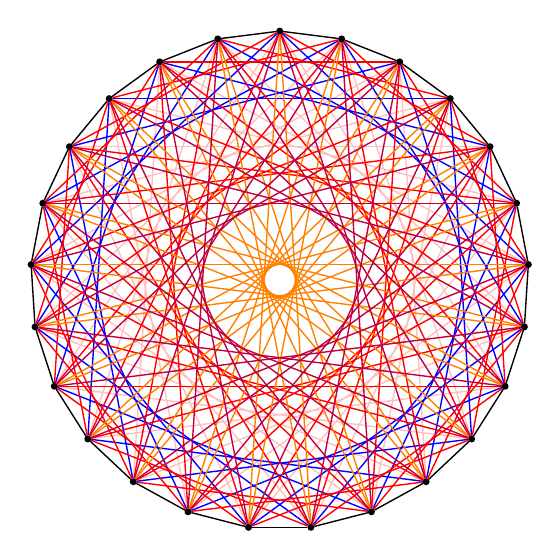
\begin{tikzpicture}[scale=.6]


\GraphInit[vstyle=Simple]
\tikzset{VertexStyle/.append style = {minimum size =2pt, inner sep = 0pt}}


\Vertex[x=187.5pt,y=337.5pt]{0};
\Vertex[x=224.80348307472823pt,y=332.7874741692947pt]{1};
\Vertex[x=259.7630511152573pt,y=318.94600200657953pt]{2};
\Vertex[x=290.1820658893033pt,y=296.8452941132117pt]{3};
\Vertex[x=314.14918882530225pt,y=267.87401924684946pt]{4};
\Vertex[x=330.15847744427305pt,y=233.85254915624213pt]{5};
\Vertex[x=337.2040092642407pt,y=196.91857792939703pt]{6};
\Vertex[x=334.8430876093033pt,y=159.3928028121413pt]{7};
\Vertex[x=323.22405786990294pt,y=123.63310626523908pt]{8};
\Vertex[x=303.0769864163684pt,y=91.88640153769651pt]{9};
\Vertex[x=275.667787843871pt,y=66.14745084375791pt]{10};
\Vertex[x=242.71868290270174pt,y=48.0335271167623pt]{11};
\Vertex[x=206.2999850346457pt,y=38.682794802828326pt]{12};
\Vertex[x=168.70001496535434pt,y=38.682794802828326pt]{13};
\Vertex[x=132.2813170972983pt,y=48.03352711676226pt]{14};
\Vertex[x=99.3322121561291pt,y=66.14745084375782pt]{15};
\Vertex[x=71.92301358363159pt,y=91.88640153769656pt]{16};
\Vertex[x=51.77594213009703pt,y=123.63310626523916pt]{17};
\Vertex[x=40.1569123906967pt,y=159.3928028121413pt]{18};
\Vertex[x=37.795990735759275pt,y=196.91857792939695pt]{19};
\Vertex[x=44.841522555726954pt,y=233.8525491562421pt]{20};
\Vertex[x=60.85081117469775pt,y=267.8740192468495pt]{21};
\Vertex[x=84.81793411069665pt,y=296.8452941132117pt]{22};
\Vertex[x=115.23694888474257pt,y=318.9460020065795pt]{23};
\Vertex[x=150.1965169252717pt,y=332.7874741692946pt]{24};

\SetUpEdge[lw         = .5pt,
            color      = black,
            labelcolor = black]

\Edge(24)(0)
\Edge(0)(1)
\Edge(1)(2)
\Edge(2)(3)
\Edge(3)(4)
\Edge(4)(5)
\Edge(5)(6)
\Edge(6)(7)
\Edge(7)(8)
\Edge(8)(9)
\Edge(9)(10)
\Edge(10)(11)
\Edge(11)(12)
\Edge(12)(13)
\Edge(13)(14)
\Edge(14)(15)
\Edge(15)(16)
\Edge(16)(17)
\Edge(17)(18)
\Edge(18)(19)
\Edge(19)(20)
\Edge(20)(21)
\Edge(21)(22)
\Edge(22)(23)
\Edge(23)(24)

\SetUpEdge[lw         = .5pt,
            color      =pink,
            labelcolor = black]

\Edge(0)(8)
\Edge(2)(10)
\Edge(4)(12)
\Edge(6)(14)
\Edge(8)(16)
\Edge(10)(18)
\Edge(12)(20)
\Edge(14)(22)
\Edge(16)(24)
\Edge(18)(1)
\Edge(20)(3)
\Edge(22)(5)
\Edge(24)(7)
\Edge(1)(9)
\Edge(3)(11)
\Edge(5)(13)
\Edge(7)(15)
\Edge(9)(17)
\Edge(11)(19)
\Edge(13)(21)
\Edge(15)(23)
\Edge(17)(0)
\Edge(19)(2)
\Edge(21)(4)
\Edge(23)(6)

\SetUpEdge[lw         = .5pt,
            color      =blue,
            labelcolor = black]

\Edge(0)(6)
\Edge(6)(12)
\Edge(12)(18)
\Edge(18)(24)
\Edge(24)(5)
\Edge(5)(11)
\Edge(11)(17)
\Edge(17)(23)
\Edge(23)(4)
\Edge(4)(10)
\Edge(10)(16)
\Edge(16)(22)
\Edge(22)(3)
\Edge(3)(9)
\Edge(9)(15)
\Edge(15)(21)
\Edge(21)(2)
\Edge(2)(8)
\Edge(8)(14)
\Edge(14)(20)
\Edge(20)(1)
\Edge(1)(7)
\Edge(7)(13)
\Edge(13)(19)
\Edge(19)(0)

\SetUpEdge[lw         = .5pt,
            color      =red,
            labelcolor = black]

\Edge(0)(4)
\Edge(4)(8)
\Edge(8)(12)
\Edge(12)(16)
\Edge(16)(20)
\Edge(20)(24)
\Edge(24)(3)
\Edge(3)(7)
\Edge(7)(11)
\Edge(11)(15)
\Edge(15)(19)
\Edge(19)(23)
\Edge(23)(2)
\Edge(2)(6)
\Edge(6)(10)
\Edge(10)(14)
\Edge(14)(18)
\Edge(18)(22)
\Edge(22)(1)
\Edge(1)(5)
\Edge(5)(9)
\Edge(9)(13)
\Edge(13)(17)
\Edge(17)(21)
\Edge(21)(0)
\Edge(0)(9)
\Edge(9)(18)
\Edge(18)(2)
\Edge(2)(11)
\Edge(11)(20)
\Edge(20)(4)
\Edge(4)(13)
\Edge(13)(22)
\Edge(22)(6)
\Edge(6)(15)
\Edge(15)(24)
\Edge(24)(8)
\Edge(8)(17)
\Edge(17)(1)
\Edge(1)(10)
\Edge(10)(19)
\Edge(19)(3)
\Edge(3)(12)
\Edge(12)(21)
\Edge(21)(5)
\Edge(5)(14)
\Edge(14)(23)
\Edge(23)(7)
\Edge(7)(16)
\Edge(16)(0)


\SetUpEdge[lw         = .5pt,
            color      = orange,
            labelcolor = black]

\Edge(24)(12)
\Edge(0)(13)
\Edge(1)(14)
\Edge(2)(15)
\Edge(3)(16)
\Edge(4)(17)
\Edge(5)(18)
\Edge(6)(19)
\Edge(7)(20)
\Edge(8)(21)
\Edge(9)(22)
\Edge(10)(23)
\Edge(11)(24)
\Edge(12)(0)
\Edge(13)(1)
\Edge(14)(2)
\Edge(15)(3)
\Edge(16)(4)
\Edge(17)(5)
\Edge(18)(6)
\Edge(19)(7)
\Edge(20)(8)
\Edge(21)(9)
\Edge(22)(10)
\Edge(23)(11)


\SetUpEdge[lw         = .5pt,
            color      = purple,
            labelcolor = black]

\Edge(24)(9)
\Edge(0)(10)
\Edge(1)(11)
\Edge(2)(12)
\Edge(3)(13)
\Edge(4)(14)
\Edge(5)(15)
\Edge(6)(16)
\Edge(7)(17)
\Edge(8)(18)
\Edge(9)(19)
\Edge(10)(20)
\Edge(11)(21)
\Edge(12)(22)
\Edge(13)(23)
\Edge(14)(24)
\Edge(15)(0)
\Edge(16)(1)
\Edge(17)(2)
\Edge(18)(3)
\Edge(19)(4)
\Edge(20)(5)
\Edge(21)(6)
\Edge(22)(7)
\Edge(23)(8)

\end{tikzpicture}
\end{center}

\begin{itemize}
		\item<1->
\begin{center}
Cay($\mathbb{Z}_{25}$, \{$\pm$1,$\pm$4,$\pm$6,$\pm$8, $\pm10$, $\pm$13\})     
\end{center}
                 
\end{itemize}
}

\frame{
\frametitle{\underline{New lower bound of $m(d, 4)$}}

\begin{theorem} As $d\to\infty$, 
\[
m(d,4) \geq \frac{512}{243}\left(\frac d4\right)^4 + O(d^3)\approx 2.106996 \left(\frac d4\right)^4 + O(d^3).
\]
\end{theorem}

}

\frame{
\frametitle{\underline{New lower bound of $m(d, 4)$}}

Let $d \geq 11$ be an integer and let $\lambda = \left \lfloor \frac{d - 2}{9} \right \rfloor$. Define
\begin{align*}
\alpha &= 3 \lambda,\\
\beta &=3 \lambda \alpha,\\
\gamma &= 3 \lambda \beta,\\
m &= 2 \lambda \gamma + \lambda \beta + \lambda \alpha + \lambda.
\end{align*}}


\frame{
\frametitle{\underline{New lower bound of $m(d, 4)$}}
Let $A = \{1, \alpha, \beta, \gamma\}$. Then
\begin{align*}
m &= 2 \lambda d + \lambda c + \lambda b + \lambda \\
&= 54\lambda^4 + 9\lambda^3 + 3\lambda^2 + \lambda\\
&= \frac{512}{243}\left(\frac d4\right)^4 + O(d^3).
\end{align*}
}

\frame{
\frametitle{\underline{New lower bound of $m(d, 4)$}}
\setbeamercolor{uppercolgreen}{fg=white,bg=blue!85}
\setbeamercolor{lowercolgreen}{fg=black,bg=blue!10}
\begin{beamerboxesrounded}[upper=uppercolgreen,lower=lowercolgreen,shadow=true]
{Definition} 
Let $dA$ denote the set of all sums of at most $d$ not necessarily distinct elements of a generating set $A$ of $\Z_m$.  
\end{beamerboxesrounded}
\vspace{5mm}
\only<1>{
	\begin{itemize}
                  \item<1-> For this proof we need to show that $dA = \Z_m$ such that the Cayley digraph Cay$(m, A)$ has diameter $d(m, A) \leq d$. 
	\end{itemize}
}

}

\frame{
\frametitle{\underline{New lower bound of $m(d, 4)$}}
Every integer $n$ such that $0 \leq n < m$ can be expressed in the following way:
\[ n = w + x\alpha + y\beta + z\gamma\]
where 
\[ 0 \leq w \leq 3\lambda, \quad 0 \leq x \leq 3\lambda,\quad 0 \leq y \leq 3\lambda,\quad 0 \leq z \leq 2\lambda.\]
}

\frame{
\frametitle{\underline{New lower bound of $m(d, 4)$}}
Thus we only need to show, for every $0 \leq n < m$, there exists nonnegative integers $\delta_1$, $\delta_2$, $\delta_3$, and $\delta_4$ such that we can write $n$ as
\[ n \equiv \delta_1 + \delta_2 \alpha + \delta_3 \beta + \delta_4 \gamma\]
where 
\[ \delta_1 + \delta_2 + \delta_3 + \delta_4 \leq d.\]

\only<1>{
	\begin{itemize}
                  \item<1-> We now consider a few subcases:
	\end{itemize}}

}

\frame{
\frametitle{\underline{New lower bound of $m(d, 4)$: Case 1.}}
\setbeamercolor{uppercolgreen}{fg=white,bg=blue!85}
\setbeamercolor{lowercolgreen}{fg=black,bg=blue!10}
\begin{beamerboxesrounded}[upper=uppercolgreen,lower=lowercolgreen,shadow=true]
{Case 1}  
\begin{center}
 $0 \leq x_3 < \lambda$
\end{center}
\end{beamerboxesrounded}
\only<1>{
	\begin{itemize}
                  \item<1-> We now consider the a few cases:
	\end{itemize}}
}

\frame{
\frametitle{\underline{New lower bound of $m(d, 4)$: Case 1.}}
Subcase 1.a. If $2 \lambda \leq x_1 < 3 \lambda$ then $0 \leq x_0 < 2\lambda$. \\
If $0 \leq x_1 < 2 \lambda$, we have 
\[ x_0 + x_1 + x_2 + x_3 \leq 3\lambda + 2\lambda + 3\lambda + \lambda = 9\lambda \leq d, \]
which implies that $n = x_0 + x_1\alpha + x_2\beta + x_3\gamma \in dA$. \\
If $2 \lambda \leq x_1 < 3 \lambda$ and  $0 \leq x_0 < 2\lambda$, we have 
\[ x_0 + x_1 + x_2 + x_3 \leq 2\lambda + 3\lambda + 3\lambda + \lambda = 9\lambda \leq d, \]
which implies that $n = x_0 + x_1\alpha + x_2\beta + x_3\gamma \in dA$. 
}

\frame{
\frametitle{\underline{New lower bound of $m(d, 4)$: Case 1.}}
Subcase 1.b. $2 \lambda \leq x_2 < 3 \lambda$, $2 \lambda \leq x_1 < 3\lambda$, $2 \lambda \leq x_0 < 3\lambda$. \\
We have
\begin{align*}
n \equiv n + m &= x_0 + x_1\alpha + x_2\beta + x_3\gamma + \lambda + \lambda \alpha + \lambda \beta + 2 \lambda \gamma\\
&=  x_0 + \lambda + (x_1 + \lambda) \alpha + (x_2 + \lambda) \beta + (x_3 + 2 \lambda) \gamma\\ 
&=  x_0 -  2\lambda + (x_1 - 2 \lambda + 1) \alpha + (x_2 + \lambda + 1) \beta + (x_3 + 2 \lambda)
 \gamma.\\ 
\end{align*}
}

\frame{
\frametitle{\underline{New lower bound of $m(d, 4)$: Case 1.}}
Noting that
\[  x_0 -  2\lambda \geq 0, x_1 - 2 \lambda + 1 \geq 0, x_2 + \lambda + 1 \geq 0, \text{ and } x_3 + 2 \lambda \geq 0, \]
we see that 
\begin{align*}
x_0 -  2\lambda + x_1 - 2 \lambda &+ 1 + x_2 + \lambda + 1 + x_3 + 2 \lambda\\
&= x_0  + x_1 +  x_2 + x_3 -  \lambda + 2 \\
&\leq 3 \lambda + 3 \lambda + 3 \lambda + \lambda - \lambda + 2\\
&= 9 \lambda + 2 \leq d,
\end{align*}
which implies that $n = x_0 + x_1\alpha + x_2\beta + x_3\gamma \in dA$. 
}

\frame{
\frametitle{\underline{New lower bound of $m(d, 4)$: Case 2.}}
\setbeamercolor{uppercolgreen}{fg=white,bg=blue!85}
\setbeamercolor{lowercolgreen}{fg=black,bg=blue!10}
\begin{beamerboxesrounded}[upper=uppercolgreen,lower=lowercolgreen,shadow=true]
{Case 2}  
\begin{center}
 $\lambda \leq x_3 < 2\lambda$
\end{center}
\end{beamerboxesrounded}
\only<1>{
	\begin{itemize}
                  \item<1-> We now consider a few subcases:
	\end{itemize}}
}

\frame{
\frametitle{\underline{New lower bound of $m(d, 4)$: Case 2.}}
Subcase 2.a. $0 \leq x_2 < 2 \lambda.$ If $2 \lambda \leq x_1 < 3 \lambda$ then $0 \leq x_0 < 2\lambda$. \\
If $0 \leq x_1 < 2 \lambda$, we have 
\[ x_0 + x_1 + x_2 + x_3 \leq 2\lambda + 2\lambda + 2\lambda + 3\lambda = 9\lambda \leq d, \]
which implies that $n = x_0 + x_1\alpha + x_2\beta + x_3\gamma \in dA$. \\
If $2 \lambda \leq x_1 < 3 \lambda$ and  $0 \leq x_0 < 2\lambda$, we have 
\[ x_0 + x_1 + x_2 + x_3 \leq 2\lambda + 2\lambda + 3\lambda + 2 \lambda = 9\lambda \leq d, \]
which implies that $n = x_0 + x_1\alpha + x_2\beta + x_3\gamma \in dA$. 
}

\frame{
\frametitle{\underline{New lower bound of $m(d, 4)$: Case 2.}}
Subcase 2.b. $\lambda \leq x_2 < 2 \lambda$, $2 \lambda \leq x_1 < 3\lambda$,  $2\lambda \leq x_0 < 3\lambda$. \\
We have
\begin{align*}
n \equiv n + m &= x_0 + x_1\alpha + x_2\beta + x_3\gamma + \lambda + \lambda \alpha + \lambda \beta + 2 \lambda \gamma\\
&=  x_0 + \lambda + (x_1 + \lambda) \alpha + (x_2 + \lambda) \beta + (x_3 + 2 \lambda) \gamma\\ 
&=  x_0 -  2\lambda + (x_1 - 2 \lambda + 1) \alpha + (x_2 + \lambda + 1) \beta + (x_3 + 2 \lambda)
 \gamma.
\end{align*}
}

\frame{
\frametitle{\underline{New lower bound of $m(d, 4)$: Case 2.}}
Noting that
\[  x_0 -  2\lambda \geq 0, \  x_1 - 2 \lambda + 1 \geq 0,  \ x_2 + \lambda + 1 \geq 0, \text{ and } x_3 + 2 \lambda \geq 0, \]
we see that 
\begin{align*}
x_0 -  2\lambda + x_1 - 2 \lambda + 1 + x_2 &+ \lambda + 1 + x_3 + 2 \lambda \\
&= x_0  + x_1 +  x_2 + x_3 -  \lambda + 2 \\
&\leq 3 \lambda + 3 \lambda + 2 \lambda + 2\lambda - \lambda + 2\\
&= 9 \lambda + 2 \leq d,
\end{align*}
which implies that $n = x_0 + x_1\alpha + x_2\beta + x_3\gamma \in dA$. 
}

\frame{
\frametitle{\underline{New lower bound of $m(d, 4)$: Case 2.}}
Subcase 2.c. $2 \lambda \leq x_2 < 3 \lambda.$ If $ \lambda \leq x_1 < 2 \lambda$ then $0 \leq x_0 < 2\lambda$. \\
If $0 \leq x_1 < \lambda$, we have 
\[ x_0 + x_1 + x_2 + x_3 \leq 3\lambda + \lambda + 3 \lambda + 2\lambda = 9\lambda \leq d, \]
which implies that $n = x_0 + x_1\alpha + x_2\beta + x_3\gamma \in dA$. \\
If $ \lambda \leq x_1 < 2 \lambda$ and  $0 \leq x_0 < 2\lambda$, we have 
\[ x_0 + x_1 + x_2 + x_3 \leq 2\lambda + 2\lambda + 3\lambda + 2 \lambda = 9\lambda \leq d, \]
which implies that $n = x_0 + x_1\alpha + x_2\beta + x_3\gamma \in dA$. 
}

\frame{
\frametitle{\underline{New lower bound of $m(d, 4)$: Case 2.}}
Subcase 2.d. $2\lambda \leq x_2 < 3 \lambda$, $ \lambda \leq x_1 < 2\lambda$,  $2\lambda \leq x_0 < 3\lambda$. \\
We have
\begin{align*}
n \equiv n + m &= x_0 + x_1\alpha + x_2\beta + x2_3\gamma + \lambda + \lambda \alpha + \lambda \beta + 2 \lambda \gamma\\
&=  x_0 + \lambda + (x_1 + \lambda) \alpha + (x_2 + \lambda) \beta + (x_3 + 2 \lambda) \gamma\\ 
&=  x_0 -  2\lambda + (x_1 + \lambda + 1) \alpha + (x_2 - 2 \lambda) \beta + (x_3 + 2 \lambda + 1)
 \gamma.
\end{align*}
}

\frame{
\frametitle{\underline{New lower bound of $m(d, 4)$: Case 2.}}
Noting that
\[  x_0 -  2\lambda \geq 0,  \ x_1 + \lambda + 1 \geq 0, \  x_2 - 2 \lambda \geq 0, \text{ and } x_3 + 2 \lambda + 1 \geq 0, \]
we see that 
\begin{align*}
x_0 -  2\lambda + x_1 + \lambda + 1 + x_2  &- 2 \lambda + x_3 + 2 \lambda + 1\\
 &= x_0  + x_1 +  x_2 + x_3 -  \lambda + 2 \\
&\leq 3 \lambda + 2 \lambda + 3 \lambda + 2\lambda - \lambda + 2\\
&= 9 \lambda + 2 \leq d,
\end{align*}
which implies that $n = x_0 + x_1\alpha + x_2\beta + x_3\gamma \in dA$. 
}

\frame{
\frametitle{\underline{New lower bound of $m(d, 4)$: Case 2.}}
Subcase 2.e. $2\lambda \leq x_2 < 3 \lambda$, $ 2\lambda \leq x_1 < 3\lambda$,  $0 \leq x_0 < 2\lambda$. \\
We have
\begin{align*}
n \equiv n + m \\
&= x_0 + x_1\alpha + x_2\beta + x_3\gamma + \lambda + \lambda \alpha + \lambda \beta + 2 \lambda \gamma \\
&=  x_0 + \lambda + (x_1 + \lambda) \alpha + (x_2 + \lambda) \beta + (x_3 + 2 \lambda) \gamma\\ 
&=  x_0 +  \lambda + (x_1 - 2 \lambda) \alpha + (x_2 - 2 \lambda + 1) \beta + (x_3 + 2 \lambda + 1)\gamma.
\end{align*}
}

\frame{
\frametitle{\underline{New lower bound of $m(d, 4)$: Case 2.}}
Noting that
\[  x_0 +  \lambda \geq 0,  \ x_1 - 2 \lambda \geq 0, \  x_2 - 2 \lambda + 1 \geq 0, \text{ and } x_3 + 2 \lambda + 1 \geq 0, \]
we see that 
\begin{align*}
x_0 + \lambda + x_1 - 2 \lambda + x_2  &- 2 \lambda + 1 + x_3 + 2 \lambda + 1 \\ 
&= x_0  + x_1 +  x_2 + x_3 -  \lambda + 2 \\
&\leq 2 \lambda + 3 \lambda + 3 \lambda + 2\lambda -  \lambda + 2\\
&= 9 \lambda + 2 \leq d,
\end{align*}
which implies that $n = x_0 + x_1\alpha + x_2\beta + x_3\gamma \in dA$. 
}


\frame{
\frametitle{\underline{New lower bound of $m(d, 4)$: Case 2.}}
Subcase 2.f. $2\lambda \leq x_2 < 3 \lambda$, $ 2\lambda \leq x_1 < 3\lambda$,  $2\lambda \leq x_0 < 3\lambda$. \\
We have
\begin{align*}
n \equiv n &+ m \\
&= x_0 + x_1\alpha + x_2\beta + x_3\gamma + \lambda + \lambda \alpha + \lambda \beta + 2 \lambda \gamma\\
&=  x_0 + \lambda + (x_1 + \lambda) \alpha + (x_2 + \lambda) \beta + (x_3 + 2 \lambda) \gamma\\ 
&=  x_0 -  2\lambda + (x_1 - 2 \lambda + 1) \alpha + (x_2 - 2 \lambda + 1) \beta + (x_3 + 2 \lambda + 1)\gamma.
\end{align*}
}

\frame{
\frametitle{\underline{New lower bound of $m(d, 4)$: Case 2.}}
Noting that
\[  x_0 -  2\lambda \geq 0,  \ x_1 - 2 \lambda + 1 \geq 0, \  x_2 - 2 \lambda + 1 \geq 0, \text{ and } x_3 + 2 \lambda + 1 \geq 0, \]
we see that 
\begin{align*}
x_0 -  2\lambda + x_1 - 2 \lambda + 1 + x_2 &- 2 \lambda + 1 + x_3 + 2 \lambda + 1 \\
&= x_0  + x_1 +  x_2 + x_3 -  4 \lambda + 3 \\
&\leq 3 \lambda + 3 \lambda + 3 \lambda + 2\lambda - 4 \lambda + 3\\
&= 7 \lambda + 2 \leq d,
\end{align*}
which implies that $n = x_0 + x_1\alpha + x_2\beta + x_3\gamma \in dA$. 
}

\frame{
\frametitle{\underline{New lower bound of $m(d, 4)$: Case 3.}}
\setbeamercolor{uppercolgreen}{fg=white,bg=blue!85}
\setbeamercolor{lowercolgreen}{fg=black,bg=blue!10}
\begin{beamerboxesrounded}[upper=uppercolgreen,lower=lowercolgreen,shadow=true]
{Case 3}  
\begin{center}
 $2\lambda \leq x_3 < 3\lambda$
\end{center}
\end{beamerboxesrounded}
\only<1>{
	\begin{itemize}
                  \item<1-> We now consider a few subcases:
	\end{itemize}}
}

\frame{
\frametitle{\underline{New lower bound of $m(d, 4)$: Case 3.}}
Subcase 3.a. $0 \leq x_2 <  \lambda.$ If $2 \lambda \leq x_1 < 3 \lambda$ then $0 \leq x_0 < 2\lambda$. \\
If $0 \leq x_1 < 2\lambda$, we have 
\[ x_0 + x_1 + x_2 + x_3 \leq 3 \lambda + 2 \lambda + \lambda + 3\lambda = 9\lambda \leq d, \]
which implies that $n = x_0 + x_1\alpha + x_2\beta + x_3\gamma \in dA$. \\
If $2 \lambda \leq x_1 < 3 \lambda$ and  $0 \leq x_0 < 2\lambda$, we have 
\[ x_0 + x_1 + x_2 + x_3 \leq 2\lambda + 3\lambda + \lambda + 3 \lambda = 9\lambda \leq d, \]
which implies that $n = x_0 + x_1\alpha + x_2\beta + x_3\gamma \in dA$. 
}

\frame{
\frametitle{\underline{New lower bound of $m(d, 4)$: Case 3.}}
Subcase 3.b. $0 \leq x_2 <  \lambda$, $ 2\lambda \leq x_1 < 3\lambda$,  $2 \lambda \leq x_0 < 3\lambda$. \\
We have
\begin{align*}
n \equiv n + m &= x_0 + x_1\alpha + x_2\beta + x_3\gamma + \lambda + \lambda \alpha + \lambda \beta + 2 \lambda \gamma\\
&=  x_0 + \lambda + (x_1 + \lambda) \alpha + (x_2 + \lambda) \beta + (x_3 + 2 \lambda) \gamma\\ 
&=  x_0 -  2\lambda + (x_1 - 2 \lambda + 1) \alpha + (x_2 + \lambda + 1) \beta + (x_3 + 2 \lambda )\gamma.
\end{align*}}

\frame{
\frametitle{\underline{New lower bound of $m(d, 4)$: Case 3.}}
Noting that
\[  x_0 -  2\lambda \geq 0,  \ x_1 - 2 \lambda + 1 \geq 0, \  x_2 + \lambda + 1 \geq 0, \text{ and } x_3 + 2 \lambda \geq 0, \]
we see that 
\begin{align*}
x_0 -  2\lambda + x_1 - 2 \lambda + 1 &+ x_2  + \lambda + 1 + x_3 + 2 \lambda \\
&= x_0  + x_1 +  x_2 + x_3 -  \lambda + 2 \\
&\leq 3 \lambda + 3 \lambda + \lambda + 3\lambda - \lambda + 2\\
&= 9 \lambda + 2 \leq d,
\end{align*}
which implies that $n = x_0 + x_1\alpha + x_2\beta + x_3\gamma \in dA$.
}

\frame{
\frametitle{\underline{New lower bound of $m(d, 4)$: Case 3.}}
Subcase 3.c. $\lambda \leq x_2 < 2 \lambda$ and $0 \leq x_1 < 2\lambda$.  If $\lambda \leq x_1 < 2 \lambda$ then $0 \leq x_0 < \lambda$. \\
If $0 \leq x_1 < \lambda$, we have 
\[ x_0 + x_1 + x_2 + x_3 \leq 3\lambda + \lambda + 2\lambda + 3\lambda = 9\lambda \leq d, \]
which implies that $n = x_0 + x_1\alpha + x_2\beta + x_3\gamma \in dA$. \\
If $ \lambda \leq x_1 < 2 \lambda$ and  $0 \leq x_0 < \lambda$, we have 
\[ x_0 + x_1 + x_2 + x_3 \leq \lambda + 2\lambda + 2 \lambda + 3 \lambda = 8\lambda \leq d, \]
which implies that $n = x_0 + x_1\alpha + x_2\beta + x_3\gamma \in dA$.
}

\frame{
\frametitle{\underline{New lower bound of $m(d, 4)$}}
Thus we have shown that every element $0 \leq n < m$ is contained in $dA$, which implies the diameter of the Cayley digraph Cay$(\Z_m, A)$ is less than or equal to $d$. 
Hence,
\[
m(d, 4) \geq2.048 \left(\frac{d}{4}\right)^4  +O(d^3)\qquad\text{as}\quad d\to\infty. \qedhere
\]

}

\end{document}